\documentclass[../Main.tex]{subfiles}
\begin{document}
\section{System's characteristics}
This study examines the efficacy and adaptability of a system that utilizes conventional social login methods to augment the UX of DApps. The following characteristics can be more detailed: \\
\indent\textbf{Security} - combining the potential benefits of blockchain smart-contract, SSS, and Pedersen DKG protocol. The security infrastructure of the system is established upon the utilization of blockchain smart contracts. Programmable contracts, operating on a decentralized network, guarantee the attributes of transparency, immutability, and tamper-proof execution of operations. Shamir secret sharing is used to fortify the protection of cryptographic keys and other forms of private information. This method entails breaking up a secret into smaller pieces and giving them to several parties. The Petersen DKG protocol distributes and secures cryptographic key generation, ensuring system security. This system lets a group of people generate a shared cryptographic key without anyone having the full key. 

\indent\textbf{Efficacy and adaptability} - By leveraging blockchain's decentralized nature, Web3Auth eliminates the reliance on centralized identity providers, reducing the potential for single points of failure and enhancing security. Additionally, blockchain-based identity systems enable instant verification of user credentials, eliminating the need for lengthy verification processes and reducing transaction times. The open solution's architecture enables seamless integration with any DApps, making it easier for developers to adopt and implement with their products. 

\indent\textbf{User-friendly} - This solution supports popular authentication mechanisms such as social login which are widely used in the traditional web. This familiarity allows users to leverage their existing accounts and authentication methods, reducing the learning curve and providing a seamless transition into the Web3 space. Users can easily authenticate their identities across multiple DApps using a unified and standardized protocol, without the need to remember and manage multiple usernames and passwords. This eliminates the hassle of creating and maintaining numerous accounts, making the user experience more streamlined and efficient.

\indent\textbf{Scalability} - Compatible with any type of social authentication, including Facebook, Google, and Twitter. Utilizing a decentralized architecture increased the request's performance and volume by spreading it across multiple executors and parallel handling processes.
\newpage
\section{Overall of system}
\begin{figure}[H]
 \centering
 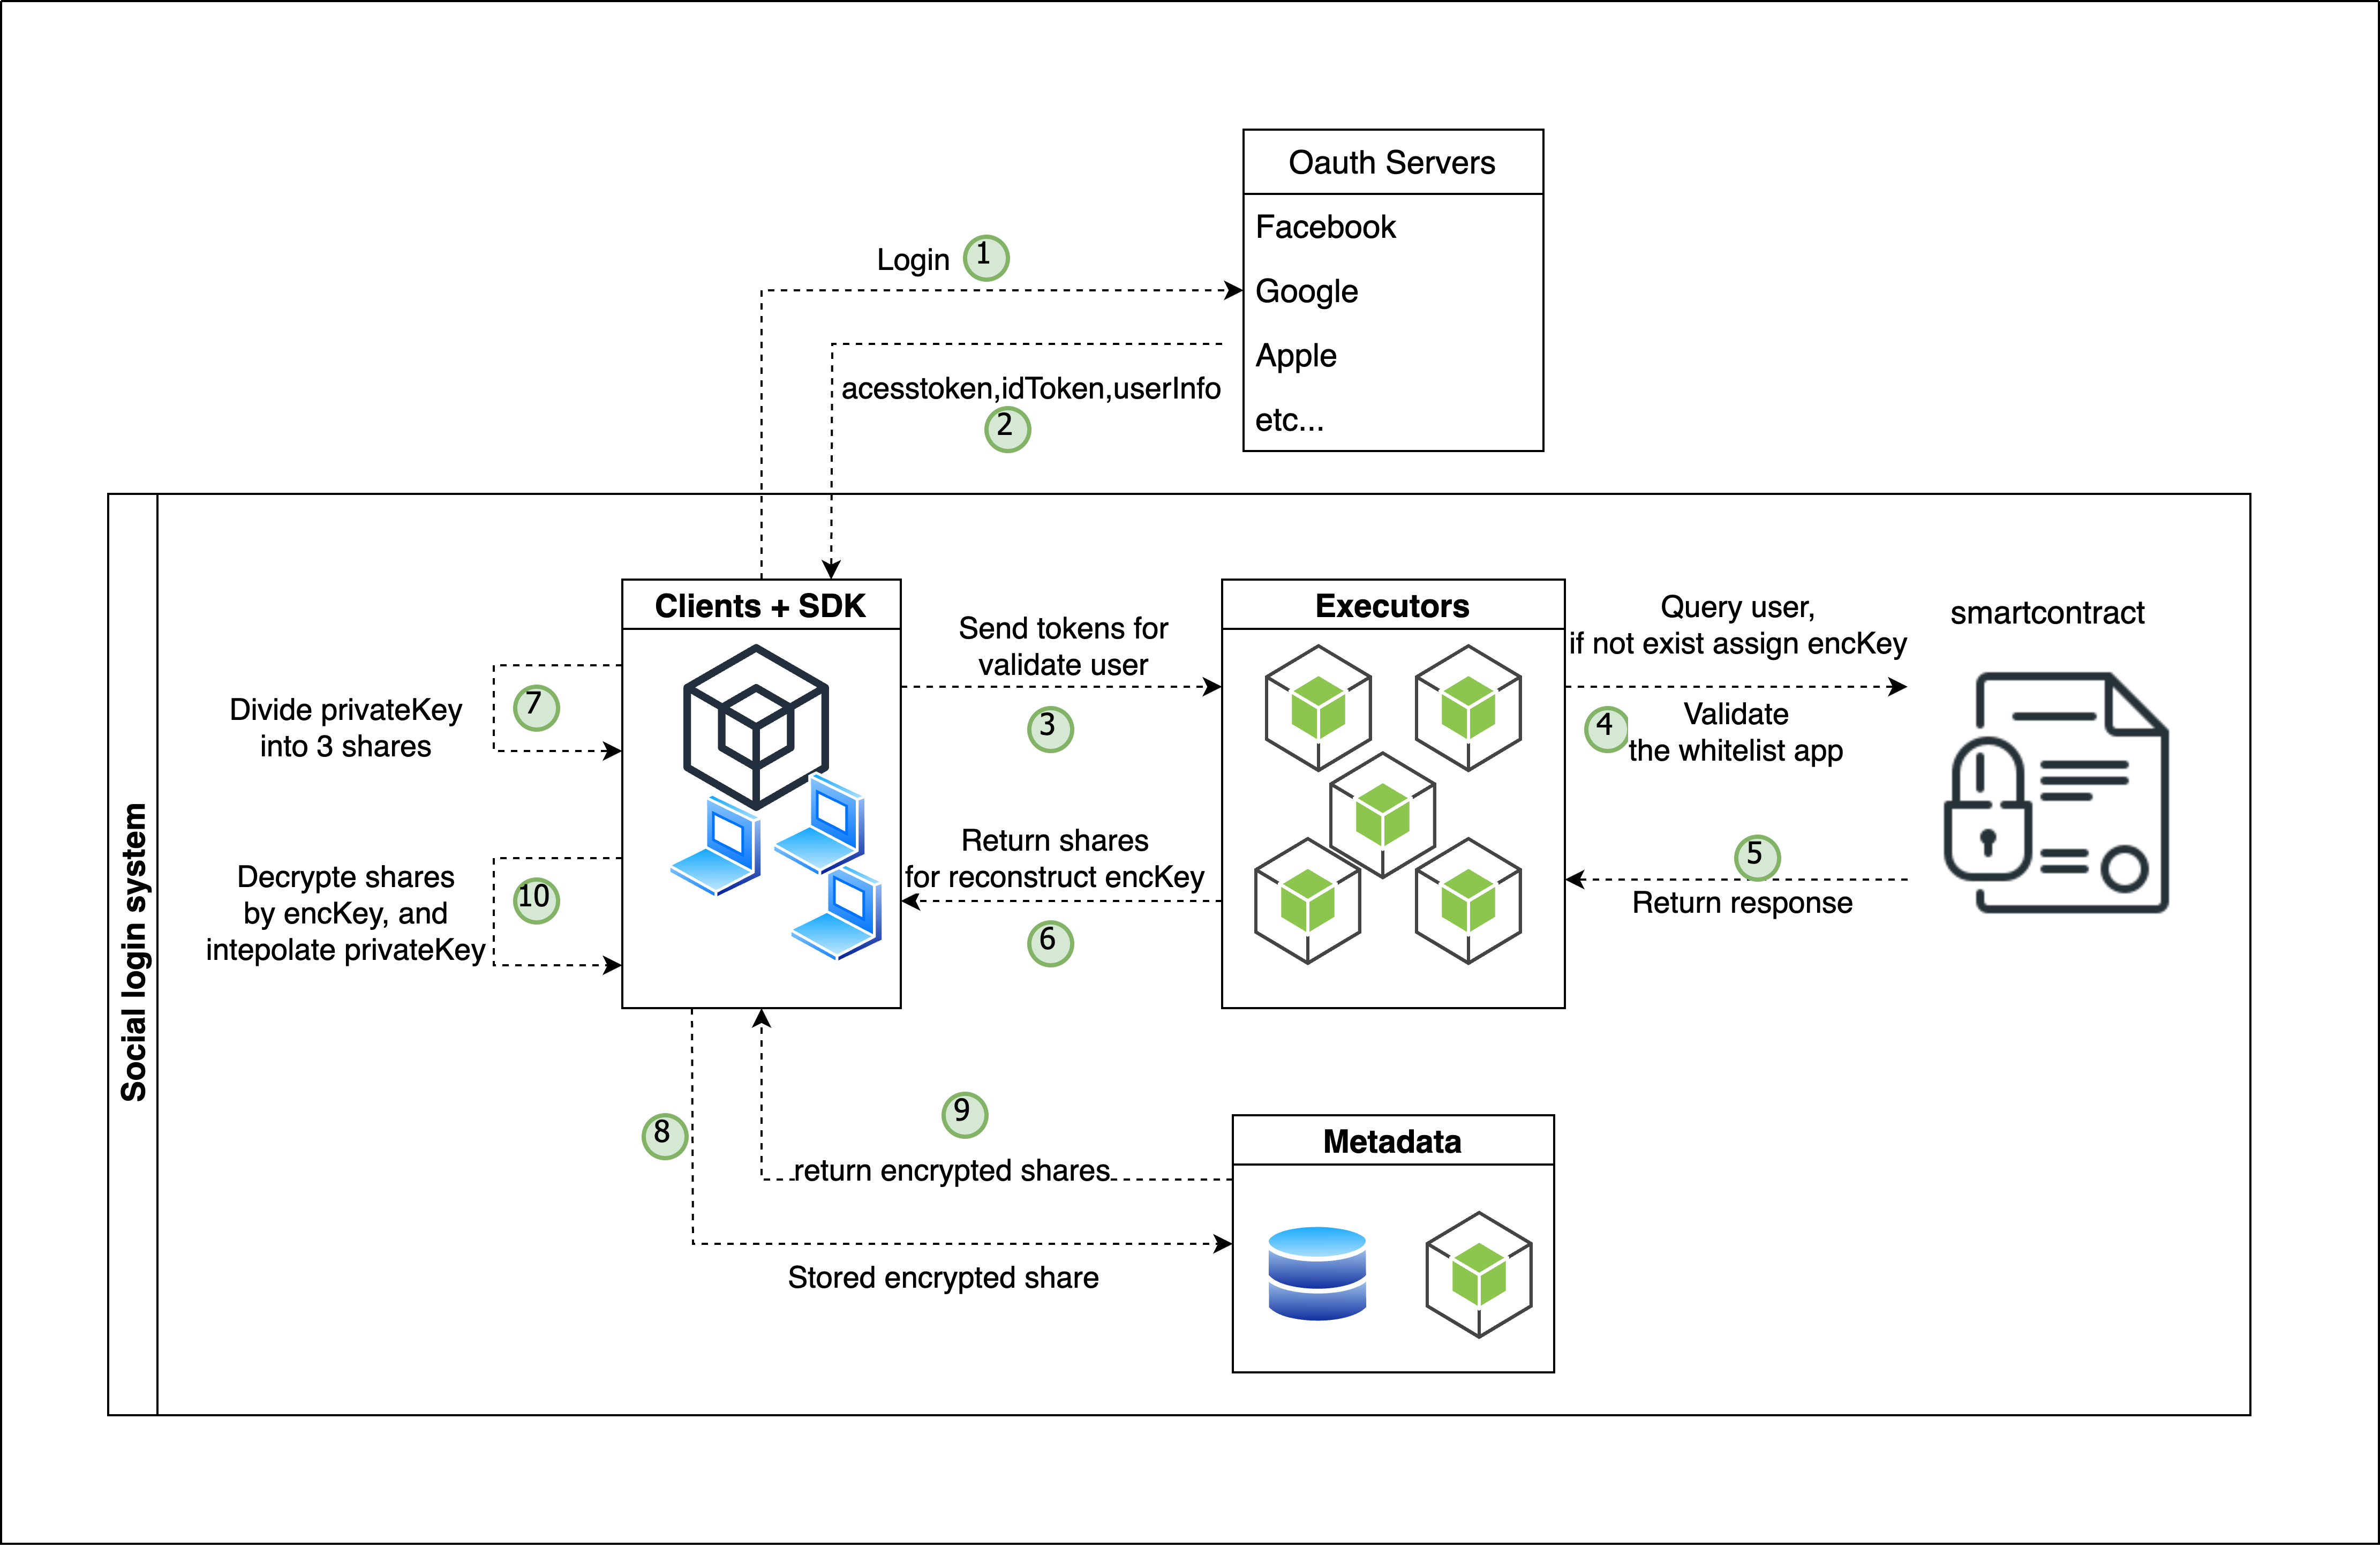
\includegraphics[scale=0.1]{Figure/OverallSocialLoginSystem.png}
    \caption{Overall the system}
    \label{fig:OverallSystem}
\end{figure}
Figure \ref{fig:OverallSystem} depicts the overall processing of a request from a user utilizing the social login system. Because the process is more complex, it has been divided into three sub-processes for clarity.

\section{Oauth2 connection}
\section{Requesting encKey for Executors}
\section{Generating and Storing Shares in Metadata}
\section{The Contribution of Executors to Pedersen's DKG Protocol}
\end{document}
